% This is LLNCS.DEM the demonstration file of
% the LaTeX macro package from Springer-Verlag
% for Lecture Notes in Computer Science,
% version 2.4 for LaTeX2e as of 16. April 2010
%
\documentclass{llncs}
%
\usepackage{makeidx}  % allows for indexgeneration
\usepackage{graphicx}
\usepackage{subfigure}
%
\begin{document}
%
\frontmatter          % for the preliminaries
%
\pagestyle{headings}  % switches on printing of running heads
\addtocmark{Hamiltonian Mechanics} % additional mark in the TOC
%
\chapter*{Preface}
%
This textbook is intended for use by students of physics, physical
chemistry, and theoretical chemistry. The reader is presumed to have a
basic knowledge of atomic and quantum physics at the level provided, for
example, by the first few chapters in our book {\it The Physics of Atoms
and Quanta}. The student of physics will find here material which should
be included in the basic education of every physicist. This book should
furthermore allow students to acquire an appreciation of the breadth and
variety within the field of molecular physics and its future as a
fascinating area of research.

For the student of chemistry, the concepts introduced in this book will
provide a theoretical framework for that entire field of study. With the
help of these concepts, it is at least in principle possible to reduce
the enormous body of empirical chemical knowledge to a few basic
principles: those of quantum mechanics. In addition, modern physical
methods whose fundamentals are introduced here are becoming increasingly
important in chemistry and now represent indispensable tools for the
chemist. As examples, we might mention the structural analysis of
complex organic compounds, spectroscopic investigation of very rapid
reaction processes or, as a practical application, the remote detection
of pollutants in the air.

\vspace{1cm}
\begin{flushright}\noindent
April 1995\hfill Walter Olthoff\\
Program Chair\\
ECOOP'95
\end{flushright}
%
\chapter*{Organization}
ECOOP'95 is organized by the department of Computer Science, Univeristy
of \AA rhus and AITO (association Internationa pour les Technologie
Object) in cooperation with ACM/SIGPLAN.
%
\section*{Executive Commitee}
\begin{tabular}{@{}p{5cm}@{}p{7.2cm}@{}}
Conference Chair:&Ole Lehrmann Madsen (\AA rhus University, DK)\\
Program Chair:   &Walter Olthoff (DFKI GmbH, Germany)\\
Organizing Chair:&J\o rgen Lindskov Knudsen (\AA rhus University, DK)\\
Tutorials:&Birger M\o ller-Pedersen\hfil\break
(Norwegian Computing Center, Norway)\\
Workshops:&Eric Jul (University of Kopenhagen, Denmark)\\
Panels:&Boris Magnusson (Lund University, Sweden)\\
Exhibition:&Elmer Sandvad (\AA rhus University, DK)\\
Demonstrations:&Kurt N\o rdmark (\AA rhus University, DK)
\end{tabular}
%
\section*{Program Commitee}
\begin{tabular}{@{}p{5cm}@{}p{7.2cm}@{}}
Conference Chair:&Ole Lehrmann Madsen (\AA rhus University, DK)\\
Program Chair:   &Walter Olthoff (DFKI GmbH, Germany)\\
Organizing Chair:&J\o rgen Lindskov Knudsen (\AA rhus University, DK)\\
Tutorials:&Birger M\o ller-Pedersen\hfil\break
(Norwegian Computing Center, Norway)\\
Workshops:&Eric Jul (University of Kopenhagen, Denmark)\\
Panels:&Boris Magnusson (Lund University, Sweden)\\
Exhibition:&Elmer Sandvad (\AA rhus University, DK)\\
Demonstrations:&Kurt N\o rdmark (\AA rhus University, DK)
\end{tabular}
%
\begin{multicols}{3}[\section*{Referees}]
V.~Andreev\\
B\"arwolff\\
E.~Barrelet\\
H.P.~Beck\\
G.~Bernardi\\
E.~Binder\\
P.C.~Bosetti\\
Braunschweig\\
F.W.~B\"usser\\
T.~Carli\\
A.B.~Clegg\\
G.~Cozzika\\
S.~Dagoret\\
Del~Buono\\
P.~Dingus\\
H.~Duhm\\
J.~Ebert\\
S.~Eichenberger\\
R.J.~Ellison\\
Feltesse\\
W.~Flauger\\
A.~Fomenko\\
G.~Franke\\
J.~Garvey\\
M.~Gennis\\
L.~Goerlich\\
P.~Goritchev\\
H.~Greif\\
E.M.~Hanlon\\
R.~Haydar\\
R.C.W.~Henderso\\
P.~Hill\\
H.~Hufnagel\\
A.~Jacholkowska\\
Johannsen\\
S.~Kasarian\\
I.R.~Kenyon\\
C.~Kleinwort\\
T.~K\"ohler\\
S.D.~Kolya\\
P.~Kostka\\
U.~Kr\"uger\\
J.~Kurzh\"ofer\\
M.P.J.~Landon\\
A.~Lebedev\\
Ch.~Ley\\
F.~Linsel\\
H.~Lohmand\\
Martin\\
S.~Masson\\
K.~Meier\\
C.A.~Meyer\\
S.~Mikocki\\
J.V.~Morris\\
B.~Naroska\\
Nguyen\\
U.~Obrock\\
G.D.~Patel\\
Ch.~Pichler\\
S.~Prell\\
F.~Raupach\\
V.~Riech\\
P.~Robmann\\
N.~Sahlmann\\
P.~Schleper\\
Sch\"oning\\
B.~Schwab\\
A.~Semenov\\
G.~Siegmon\\
J.R.~Smith\\
M.~Steenbock\\
U.~Straumann\\
C.~Thiebaux\\
P.~Van~Esch\\
from Yerevan Ph\\
L.R.~West\\
G.-G.~Winter\\
T.P.~Yiou\\
M.~Zimmer\end{multicols}
%
\section*{Sponsoring Institutions}
%
Bernauer-Budiman Inc., Reading, Mass.\\
The Hofmann-International Company, San Louis Obispo, Cal.\\
Kramer Industries, Heidelberg, Germany
%
\tableofcontents
%
\mainmatter              % start of the contributions
%
\title{Scalable Stream Clustering in Apache Spark}
%
\titlerunning{Scalable Stream Clustering in Spark}  % abbreviated title (for running head)
%                                     also used for the TOC unless
%                                     \toctitle is used
%
\author{Ivar Ekeland\inst{1} \and Roger Temam\inst{2}
Jeffrey Dean \and David Grove \and Craig Chambers \and Kim~B.~Bruce \and
Elsa Bertino}
%
\authorrunning{Ivar Ekeland et al.} % abbreviated author list (for running head)
%
%%%% list of authors for the TOC (use if author list has to be modified)
\tocauthor{Ivar Ekeland, Roger Temam, Jeffrey Dean, David Grove,
Craig Chambers, Kim B. Bruce, and Elisa Bertino}
%
\institute{Princeton University, Princeton NJ 08544, USA,\\
\email{I.Ekeland@princeton.edu},\\ WWW home page:
\texttt{http://users/\homedir iekeland/web/welcome.html}
\and
Universit\'{e} de Paris-Sud,
Laboratoire d'Analyse Num\'{e}rique, B\^{a}timent 425,\\
F-91405 Orsay Cedex, France}

\maketitle              % typeset the title of the contribution

\begin{abstract}
Two of the most popular strategies to mine big data are distributed comput-
ing and stream mining. The purpose of this thesis is to incorporate both together
bringing a competitive stream clustering method into a modern framework for
distributed computing, namely, Apache Spark. The method in question is CluS-
tream, a stream clustering method which separates the clustering process into two
different phases: an online phase which handles the incoming stream, generating
statistical summaries of the data and an offline phase which takes those summaries
to generate the final clusters. These summaries also contain valuable information
which can be used for further analysis. The main goal is to adapt this method in
such a framework in order to obtain a scalable stream clustering method which is
open source and can be used by the Apache Spark community.
\keywords{Stream mining, Clustering, CluStream}
\end{abstract}
%
\section{Introduction}


The analysis of data streams comes along with important questions: what kind of
data is it? What important information is contained in it? How does the stream
evolve? The key question for this project among those is the latter, i.e. dealing with
the evolution of the stream, because prior to the development of the CluStream \cite{clustreamOrig}
method there was not an easy to answer that question as it was one of the first to
tackle this issue.

Clustering is one of the main tasks in data mining, also often referred as an
exploratory subtask of it. As the name implies, the objective is to find clusters, i.e.,
collections of objects that share common properties. One can also relate this task
to unsupervised machine learning, which intends to classify data when it lacks of
labels, i.e., when the data instance does not indicate to which category it belongs.
The CluStream method was developed in 2003 \cite{clustreamOrig} and its main purpose is to pro-
vide more information than previously developed algorithms for data stream clus-
tering by that time. It provides a solution for handling streams of data indepen-
dently from the one that finds the final clusters. It consists of two phases (passes)
instead of one; the first one deals with the incoming data and stores relevant in-
formation over time and the second one is in charge of the clustering using the
previously generated information. In other words,

\begin{itemize}
 \item For each batch of data, statistically relevant ”summaries” of the data are cre-
ated and stored at a defined pace. This storing pace follows a specific storage
scheme such that the disk space requirement reduces drastically; this is nec-
essary as in most cases for data streams one does not want to store everything
that arrives, one reason being the big data requires large and expensive com-
putational resources (processing power and storage).
\item On user demand, the stored ”summaries” can be used for the end clustering
task as they include all necessary information to achieve accurate results.
Additionally, as these summaries are stored over time, a user defined time
horizon/window can be chosen in order to analyze the data in different time
periods, giving the possibility of a better understanding of the evolution of
the data.
\end{itemize}




\section{Related work}

\subsection{SAMOA}

\textit{CluStream} has been implemented in different types of software and libraries, being \textit{SAMOA - Scalable Advanced Massive Online Analysis} one of the options. It is also a distributed computing implementation of the algorithm. The difference is that it is not implemented in \textit{Spark}, but rather in a \textit{Distributed Stream Processing Engine} which adapts the \textit{MapReduce} approach to parallel stream processing\cite{samoa}.

Main differences with this adaptation: 

\begin{itemize}
 \item It does not include an offline macro-clustering phase.
 \item It is developed in \textit{Java} and not designed to work with Spark.
\end{itemize}

\subsection{StreamDM}

\textit{StreamDM} is a collection of algorithms for mining big data streams \footnote{As it is stated by them here: http://huawei-noah.github.io/streamDM/}. One of the included methods for stream clustering is \textit{CluStream}. This collection of algorithms is developed for Spark.

Main differences with this adaptation: 

\begin{itemize}
 \item It does not include an offline macro-clustering phase.
\end{itemize}

\section{Basic notions}

\subsection{SPARK}

\textit{Apache Spark} is an open source framework developed in the AMPLab at the University of California, campus Berkeley\cite{SparkResearch}. It is a fast and general engine for large-scale data processing, as they describe it themselves. The original goal was to design a new programming model that supports a wider class of applications than MapReduce and at the same time keeping the fault tolerance property of it. They claim MapReduce is inefficient for applications that require a multi-pass implementation and a low latency data sharing across parallel operations, which are common in data analytics nowadays, such as: 

\begin{itemize}
 \item Iterative algorithms: many machine learning and graph algorithms.
 \item Interactive data mining: multiple queries on data loaded into RAM.
 \item Streaming applications: some require an aggregate sate over time.
\end{itemize}

Traditionally, MapReduce and DAG engines are based on an acyclic data flow, which makes them non optimal for these applications listed above. In this flow, data has to be read from a stable storage system, like a distributed file system, and then processed on a series of jobs only to be written back to the stable storage. This process of reading and writing data on each step of the workflow causes a significant rise in computational cost.

The solution proposed offers \textit{resilient distributed datasets (RDDs)} to overcome this issue efficiently. RDDs are stored in memory between queries (no need of replication) and they can rebuild themselves in case of failure as they remember how they were originally built from other datasets by transformations such as \textit{map, group, join}.

\subsection{SPARK streaming}

For this project, Spark streaming plays an important role as it takes a raw data stream and transforms it so that it is possible to process it within the framework. A raw stream of data can come in different forms and through different channels: from a very simple file stream, where whenever a new file is added to a specific location it is recognized as the input, a socket stream where the data comes through the network using a TCP protocol and also integrates with more elaborated sources such as \textit{Kafka, Flume, Twitter, HDFS/S3,} etc.


\begin{figure}[h!]
 \centering
 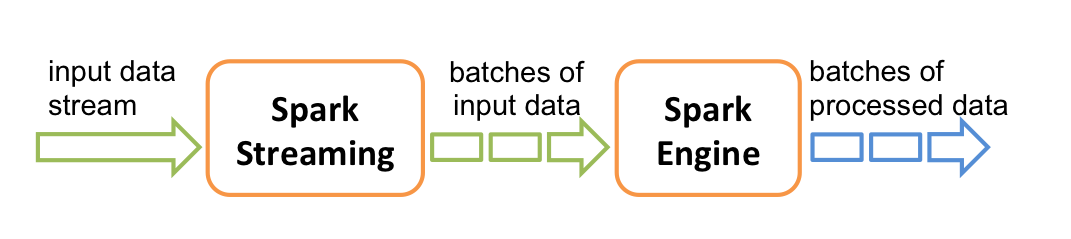
\includegraphics[scale=0.6]{./styles/streaming-flow.png}
 % streaming-flow.png: 0x0 pixel, 300dpi, 0.00x0.00 cm, bb=
 \caption{Flow of data in Spark streaming}
 \label{fig:streamFlow}
\end{figure}

Figure \ref{fig:streamFlow} shows the general idea of Spark streaming\cite{sparkStreaming}, a raw stream is linked to this module and it converts it to batches of data at user-defined intervals. These batches of data are then treated as RDDs, thus it gets distributed over the cluster where Spark runs. The abstraction of a data stream in Spark is called \textit{DStream}, which stands for Discretized Stream, and is continuous series of RDDs. In a \textit{DStream}, each RDD contains data from a specific interval of time, as it can be seen in Figure \ref{fig:dstream}.


\begin{figure}[h!]
 \centering
 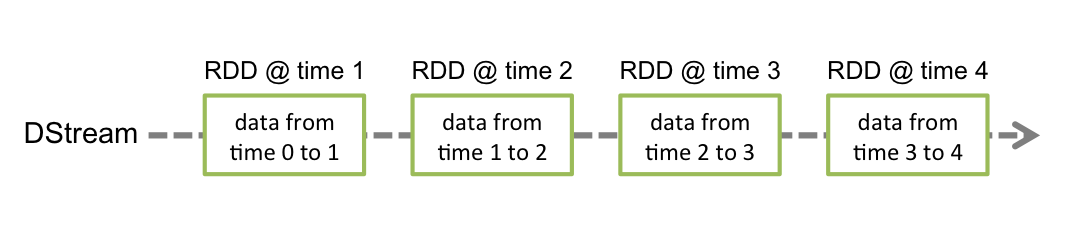
\includegraphics[scale=0.6]{./styles/streaming-dstream.png}
 % streaming-flow.png: 0x0 pixel, 300dpi, 0.00x0.00 cm, bb=
 \caption{DStreams are Spark streaming's abstraction of a data stream}
 \label{fig:dstream}
\end{figure}

\subsection{CluStream}

\textit{CluStream} is a method developed in the Watson Research Center at IBM and the University of Illinois, UIUC. This method presented a different approach on the matter of clustering streams of data with respect to a modified version of \textit{K-Means} which was adapted to work also with data streams. The main difference relies on the separation of the clustering process into two parts: one which would handle the data stream itself gathering only statistically relevant information (online part) and another which actually process the results of the former to produce the actual clusters wanted (offline part). 

Separating the clustering process provides the user several advantages, among others:

\begin{itemize}
 \item by saving only statistical data, rather than the original content, it is possible to save physical storage space (e.g. hard drive space) and therefore reducing costs and allowing a wider range in time to be clustered.
 
 \item The method also allows the analysis of the evolution of the data, as the necessary information for that is contained in the stored statistical information.
 
 \item Because the two parts operate independently it allows the user to select a time horizon, or even a time window, to perform the offline clustering part using the stored statistical information.
\end{itemize}

\subsection{The CluStream framework}

This method is built over a few ideas that need to be conceptualized, which will answer fundamental questions and set up a basis of terminology useful along this work.

\begin{itemize}
 \item \textbf{Micro-Clusters}: that is the given name for the statistical information summaries that is computed during the online component. They are a temporal extension of \textit{cluster feature vectors}\cite{zhang96birch}, which benefit from an additive feature that makes them a natural choice for the data stream problem\cite{clustreamOrig}.
 
 \item \textbf{Pyramidal time frame}: micro-clusters are stored periodically following a pyramidal pattern. This allows a nice tradeoff between the ability to store large amounts of information while giving the user the possible to work with different time horizons without loosing too much precision. The statistical summaries stored are used by the offline component to compute finally the macro-clusters which are the actual clusters the user intended to get.
\end{itemize}

It is assumed that a data stream comes in the form of multi-dimensional records $\bar X_1 ... \bar X_k ...$ where $\bar X_i = (x^1_i ... x^d_i)$.

\begin{definition}\cite{clustreamOrig}

A micro-cluster for a set of d-dimensional points $X_{i_1} ...X_{i_n}$ with time stamps
$T_{i_1} ...T_{i_n}$ is defined as the $2 \cdot d + 3)$ tuple $(\overline{CF2^x},\overline{CF1^x},CF2^t,CF1^t,n)$, wherein $\overline{CF2^x}$ and $\overline{CF1^x}$ each correspond to a vector of d entries. The definition of each of these entries is as follows: 

\begin{itemize}
 \item For each dimension, the sum of the squares of the data values is maintained in $\overline{CF2^x}$. Thus, $\overline{CF2^x}$ contains d values. The p-th entry of $\overline{CF2^x}$ is equal to $\sum^n_{j=1} (x^p_{i_j})^2$. 
 \item For each dimension, the sum of the data values is maintained in $\overline{CF1^x}$. Thus, $\overline{CF1^x}$ contains d values. The p-th entry of $\overline{CF1^x}$ is equal to $\sum^n_{j=1} x^p_{i_j}$.
 \item The sum of the squares of the time stamps $T_{i_1} ...T_{i_n}$ is maintained in $CF2^t$.
 \item The sum of the time stamps $T_{i_1} ...T_{i_n}$ is maintained in $CF1^t$.
 \item The number of data points is maintained in n.
\end{itemize}

\end{definition}

The idea behind the pyramidal time frame is that \textit{snapshots} of the micro-clusters can be stored in an efficient way, such that if $t_c$ is the current clock time and $h$ is the history length, it is still possible to find an accurate approximation of the higher level clusters (macro-clusters) for a user specified time horizon $(t_c - h, t_c)$.

In this time frame, the snapshots are stored at different levels of granularity that depends upon the \textit{recency} of them. These are classified in different orders which can vary from 1 to $log(T)$, where $T$ is the clock time elapsed since the beginning of the stream. The snapshots are maintained as follows:

\begin{itemize}
 \item A snapshot of the $i$-th order occur at time intervals $\alpha^i$, for $\alpha \geq 1$. In other words, a snapshot occurs when $T \bmod \alpha^i = 0$.
 \item At any given moment, only the last $\alpha^l + 1$ snapshot for any given order are stored, where $l \geq 1$ is a modifier which increases the accuracy of the time horizon with the cost of storing more snapshots. This allows redundancy, but from an implementation point of view only one snapshot must be kept.
 \item For a data stream, the maximum number of snapshots stored is $(\alpha^l + 1)\cdot log_{\alpha}(T)$.
 \item For any specified time window $h$, it is possible to find at least one stored snapshot within $2\cdot h$ units of the current time\footnote{The proof can be found in the original article\cite{clustreamOrig}.}.
 \item The time horizon $h$ can be approximated to a factor of $1 + (1/ \alpha^{l-1})$, whose second summand is also referred as the accuracy of the time horizon.
\end{itemize}

\begin{figure}[h!]
 \centering
 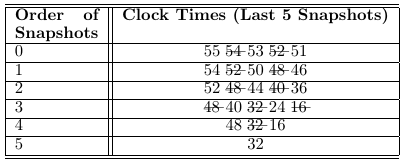
\includegraphics{./styles/pyramidalFrame.png}
 % pyramidalFrame.png: 0x0 pixel, 300dpi, 0.00x0.00 cm, bb=
 \caption{Example of snapshots stored for $\alpha = 2$ and $l=2$}
 \label{table:timeFrame}
\end{figure}

With the help of Figure \ref{table:timeFrame} it is possible to observe how this pyramidal time frame works: snapshots of order 0 occur at odd time units, these need to be retained as are non-redundant; snapshots of order 1 which occur at time units not divisible by 4 are non-redundant and must be retained; in general, all the snapshots of order $i$ which are not divisible by $\alpha^{i+1}$ are non-redundant. Another thing to note is that whenever a new snapshot of a particular order is stored, the oldest one from that order needs to be deleted.

To illustrate the effect on the accuracy of storing more snapshots, the following example is given: supposing that a stream is running for 100 years, with a time granularity of 1 second. The total number of snapshots stored would be $(2^2 + 1)\cdot log_{\alpha}(100*365*24*60*60) \approx 158$ with an accuracy of $1/ 2^{2-1} = 0.5$ or 50\% of a given time horizon $h$. Increasing the modifier $l$ to 10 would yield to $(2^{10} + 1)\cdot log_{\alpha}(100*365*24*60*60) \approx 32343$ maximum snapshots stored with an accuracy of $1/ 2^{10-1} \approx 0.00195$ or $\approx$ 0.2\% which is a significant improvement.


\subsection{Online Micro-clustering}

During this process, the incoming information is analyzed and transformed into statistical summaries that are easier to handle. This process is divided in three parts: initialization, classification and assignation, these are described as follows:

\subsubsection{Initialization}

Before the main maintenance of the micro-clusters, the initialization of $q$ micro-clusters must be performed and each of them are identified with a unique $id$. The number $q$ is taken as a user input and highly depends on the number of final macro-clusters to be calculated and the capabilities of the system where the algorithm runs. 

\begin{itemize}
 \item Random initialization:
 \begin{enumerate}
  \item generate $q$ random d-dimensional vectors to use as centroids of the micro-clusters so that data can be randomly assigned to different micro-clusters. 
  \item Assign the first incoming batch of data to their closest random centroids\footnote{See the assignation process for the details.}.
 \end{enumerate}

 \item KMeans initialization:
 \begin{enumerate}
  \item take the first $n_i$ points, number which is specified by the user, and perform the KMeans clustering method  for $q$ clusters. By doing this it is possible to ensure that the first $n_i$ points will be better clustered than after a random initialization. 
  \item Assign the first incoming batch of data to their closest found centroids.
 \end{enumerate}

\end{itemize}


\subsubsection{Classification}
\label{clus:classification}
When a new batch of data arrives, it is necessary to verify point by point whether they belong to a micro-cluster or not. This means that a point has to be located within a factor $t$ of the RMS deviation\footnote{The RMSD can be obtained using $\overline{CF2^x}$ and $\overline{CF1^x}$ as shown in \ref{findingoutliers}} (RMSD) of the nearest micro-cluster, otherwise it is considered an outlier.

Outliers are taken into account as possible new micro-clusters, this is because the stream of data might change over time. To do so, one new micro-cluster should be created with an entirely new $id$, containing the outlier. The number of micro-clusters $q$ is fixed, so one micro-cluster must be freed either by deleting an old micro-cluster of by merging two of them. To decide whether a micro-cluster is safe to delete, it is necessary to compute its value of \textit{recency} (RV) and compare it to a user defined threshold $\delta$, if no micro-cluster is safe to delete, then the two closest micro-clusters are merged.

\begin{enumerate}
 \item Check if a point $X_{i_k}$ is not an outlier: $distance(\bar X_{i_k}, \hat M_j) \leq t \cdot RMSD$, where $\hat M_j$ is the nearest micro-cluster.
 \begin{itemize}
  \item If $X_{i_k}$ is an outlier: compute $RV_{M_j}$, if $N_j < 2*m$ then the mean the time stamps is used, otherwise compute an approximation for the last $m$ points of each micro-cluster assuming its points are normally distributed\footnote{It is possible to derive the mean and the standard deviation from $CF2^t$ and $CF1^t$ as shown in \ref{handlingoutliers}} for the $1 - m/2N_j$ percentile.
  \begin{enumerate}
   \item If $RV_{M_j} < T - \delta$, where $RV_{M_j}$ is the \textit{recency} value for a given micro-cluster and $T$ the current clock time units elapsed since the beginning of the stream, then $M_j$ is safe to delete and a new micro-cluster $M_{newID}$ must replace it containing $X_{i_k}$.
   \item When there is no $M_j$ safe to delete, then merge $M_j$ and $M_{jj}$ such that $min\{M_j,M_{jj} : M_j,M_{jj} \in M_Q, distance(M_j,M_{jj})\}$, where $M_Q$ is the set of all micro-clusters. The new merged micro-cluster will now have a list of IDs $\{j,jj\}$ and a new micro-cluster $M_{newID}$ must replace $M_{jj}$ containing $X_{i_k}$.
  \end{enumerate}

 \end{itemize}
 \item Assign the point $X_{i_k}$ to $\hat M_j$.

\end{enumerate}


\subsubsection{Assignation}

When a point $X_{i_k}$ is assigned to a micro-cluster, the tuple $(\overline{CF2^x},\overline{CF1^x},CF2^t,CF1^t,n)$ for $M_j$ needs to be maintained, due to its addition properties it is possible to do so directly as follows:

\begin{itemize}
 \item $\overline{CF2^x}_{new} = \overline{CF2^x}_{old} + \overline{CF2^x}_{X_{i_k}} = \overline{CF2^x}_{old}^p + (x^p_{i_k})^2\ \forall p \in \{1,2...d\}$
 \item $\overline{CF1^x}_{new} = \overline{CF1^x}_{old} + \overline{CF1^x}_{X_{i_k}} = \overline{CF2^x}_{old}^p + x^p_{i_k} \ \forall p \in \{1,2...d\}$
 \item $\overline{CF2^t}_{new} = \overline{CF2^t}_{old} + \overline{CF2^t}_{X_{i_k}} = \overline{CF2^x}_{old} + (T_{i_k})^2$
 \item $\overline{CF1^t}_{new} = \overline{CF1^t}_{old} + \overline{CF1^t}_{X_{i_k}} = \overline{CF2^x}_{old} + T_{i_k}$
 \item $n_{new} = n_{old} + 1$
\end{itemize}


\subsection{Offline Macro-Clustering} \label{cluOffline}

While the online process transforms the stream into statistical summaries in the form of micro clusters, the offline process uses this result to deliver the final micro-clusters\footnote{In K-Means this know as the $k$ clusters.} for a given time horizon. This means that the micro clusters in the snapshots stored are now the input data for the macro-clustering process.

Assuming that $t_c$ is the current time and $h$ is the user defined horizon, the time window of information would be $(t_c, t_c - h)$. Having snapshots means that probably $t_c - h$ will not exist in an exact form but the snapshot that occurred just before that time is chosen. The pyramidal time frame ensures that it is always possible to find a snapshot $t_c - h'$ within the user specified tolerance for any $h$.

If $S(t_c - h')$ is the set of micro-clusters at time $t_c - h$ and $S(t_c)$ is the set of micro-clusters at time $t_c$, it is possible to find the final set of micro-clusters $N(t_c,h')$ by subtracting from $S(t_c)$ each corresponding micro-cluster in $S(t_c - h')$. This is possible due to the fact that each micro-cluster is associated with a list of $ids$. Doing this ensures that micro-clusters created before the user specified time horizon do not dominate the the results of the clustering process. 

\begin{property}\label{prop1}
 Let $C_1$ and $C_2$ be two sets of points. Then the cluster feature vector $\overline{CFT(C_1 \cup C_2)}$ is given by of $\overline{CF2(C_1)} + \overline{CF2(C_2)}$
\end{property}

\begin{property}\label{prop2}
 Let $C_1$ and $C_2$ be two sets of points such that $C_1 \supseteq C_2$. Then the cluster feature vector $\overline{CFT(C_1 - C_2)}$ is given by $\overline{CF2(C_1)} - \overline{CF2(C_2)}$
\end{property}

Properties \ref{prop1} and \ref{prop2} show, respectively, the additive and subtractive nature of the cluster feature vectors. This is particularly helpful as only two snapshots are required to approximate any user specified time horizon or window.

Once $N(t_c,h')$ is constructed, the micro-clusters in it are treated as \textit{pseudo-points} K-Means can be used to determine the higher level and final clusters after slightly adjusting it:

\begin{itemize}
 \item At its initialization step, the seeds are sampled with probability proportional to the number of points each micro-cluster has instead of picking them randomly, which correspond to the centroids of the micro-clusters.
 \item The distance from a seed to a \textit{pseudo-point} is equal to the distance between the seed and the centroid of the corresponding micro-cluster.
 \item When the seeds are adjusted, the new seed is defined as the weighted centroid of the micro-clusters in that partition.
\end{itemize}

As a matter of fact, following the previous modifications, many traditional clustering algorithms could be used if needed.


\section{Spark-CluStream}


\section{Experiments}

\subsection{Validation}


Two cases are analyzed in this section. These cases are two of the ones used by the developers of \textit{CluStream} to test its clustering capabilities. The tests differ in two ways: the speed of the stream and the time window used. The desired result would be to obtain comparable results for \textit{Spark-CluStream}.

\subsubsection{Case 1}

The first case uses a stream speed of 2000 points per time unit and a horizon $H=1$. The dataset contains exactly 494021 points, meaning that the online phase would require $\frac{494021}{2000} \approx 247$ time units to complete.

The measurement is the sum of squares (SSQ) of the euclidean distances from the points to their nearest macro-cluster. In fact, the case is run a total of 4 times for \textit{Spark-CluStream} to compute an average. The SSQ is defined as:

\begin{equation}
 SSQ = \sum_{i=1}^N distance(p_i,c)^2,
\end{equation}

where $N$ is the number of points used in the horizon $H=1$, which should average $N \approx 2000\cdot H \approx 2000$ points.

The parameters used in \cite{clustreamOrig} are: $\alpha=2,l=10,InitNumber=2000,\delta=512,t=2$.

\begin{figure}[h]
 \centering
 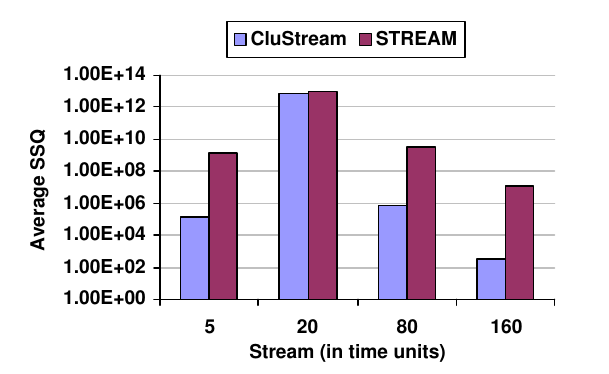
\includegraphics[scale=0.6]{./styles/2000h1-orig.png}
 % 2000h1-orig.png: 0x0 pixel, 300dpi, 0.00x0.00 cm, bb=
 \caption{Results for the original $CluStream$\cite{clustreamOrig}. Stream speed = 2000, H=1}
 \label{fig:2000orig}
\end{figure}

Figure \ref{fig:2000orig} shows the results used by the original \textit{CluStream} to show its capabilities against an older method \textit{STREAM}, which is a modified version of K-Means for data streams. The average SSQ for \textit{CluStream} is the most relevant to this test.

The parameters used for \textit{Spark-CluStream} were matched. 

\begin{figure}[h!]
 \centering
 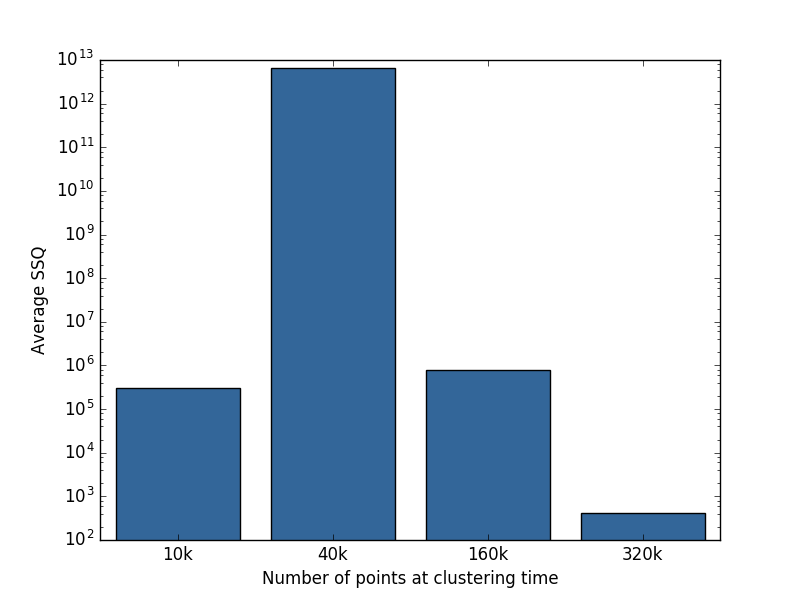
\includegraphics[scale=0.5]{./styles/2000h1.png}
 % 2000h1-orig.png: 0x0 pixel, 300dpi, 0.00x0.00 cm, bb=
 \caption{Validation results for $Spark-CluStream$. Stream speed = 2000, H=1}
 \label{fig:2000}
\end{figure}

The parameter $m$, for $m$ last points, was the only one not provided. Here, $m=20$ was chosen. For this case, both $m$ and $\delta$ are irrelevant and the reason is that the threshold is never reached (247 time units vs. 512). The number of micro-clusters $q$ is 50, a 10 times the number of final clusters (5) is enough for the vast majority of cases\cite{clustreamOrig}. The rest of the parameters were matched, with the only remaining thing to point out is that \textit{fakeKMeans()} used 5000 sampled points.

Figure \ref{fig:2000} shows the results obtained by \textit{Spark-CluStream}. There is a difference in the labels of the horizontal axis, while Figure \ref{fig:2000orig} shows the time units of the stream, Figure \ref{fig:2000orig} shows the number of points that had been streamed and processed. This is done because Spark streaming libraries in combination with the streaming simulation do not always deliver the same amount of points every single time unit, leading to inaccurate results comparing only by clustering on certain time units. A basic multiplication was used to determine the exact moment in terms of points: $2000\cdot 5 = 10000$, $2000\cdot 20 = 40000$ and so on.

Comparing the results, it is possible to deduce that they are very similar. The exact values for Figure \ref{fig:2000orig} are not available but it suffices to compare the magnitudes of the average SSQ. 

\begin{center}
\begin{tabular}{|l|l|l|l|l|}\hline
\textbf{Case 1: SSQ} & \textbf{10k} & \textbf{40k} & \textbf{160k} & \textbf{320k}\\\hline
CluStream & $10^5$-$10^6$ & $10^{12}$-$10^{13}$ & $\approx 10^6$ & $10^2$-$10^3$\\\hline
Spark-CluStream & $3.099\times10^5$ & $6.676\times10^{12}$ & $7.833\times10^5$ & $4.191\times10^2$\\\hline
\end{tabular}
\end{center}



\subsubsection{Case 2}

The second case uses a stream speed of 200 points per time unit and a horizon $H=256$. The dataset contains exactly 494021 points, meaning that the online phase would require $\frac{494021}{200} \approx 2470$ time units to complete.

The measurement is the SSQ again and the same circumstances apply for this case as in the first one with the difference that here $\delta$ and $m$ are relevant. The parameter $m$ is again chosen to be 20: if 200 points are processed every time unit and there are 50 micro-clusters, assuming all 200 points should be distributed uniformly at least every 5 time units leads to $5\frac{200}{50}=20$. An in-depth analysis of the behavior of \textit{CluStream} for different $\delta$'s and $m$'s is out of the scope of this work. 


\begin{figure}[h]
\hfill
\subfigure[\textit{Spark-CluStream}]{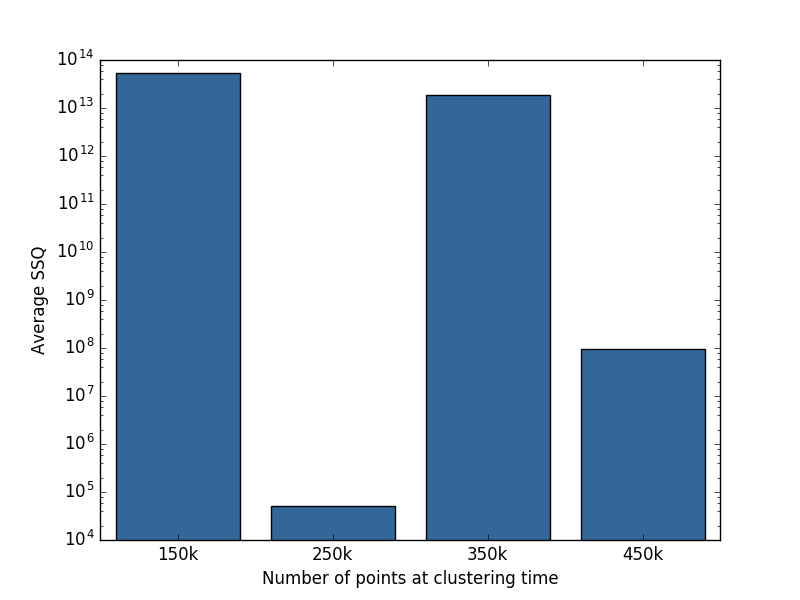
\includegraphics[width=5cm]{./styles/200h256.png}}
\hfill
\subfigure[Original \textit{CluStream}\cite{clustreamOrig}]{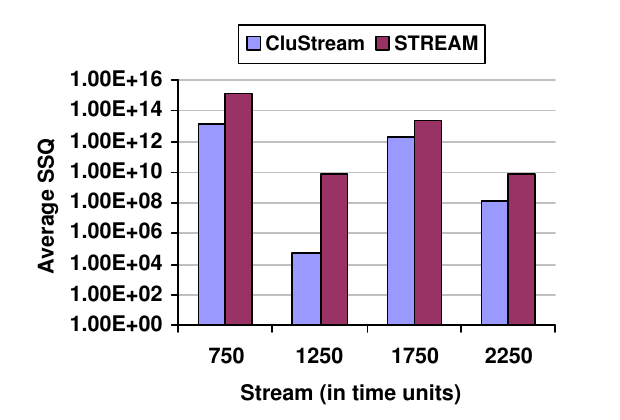
\includegraphics[width=5cm]{./styles/200h256-orig.png}}
\hfill
\caption{Validation results: case 2. Stream speed = 200, H = 256}
\label{fig:200h256}
\end{figure}

Again, the comparison is for the average SSQ. The test ran 4 times for \textit{Spark-CluStream} to average the results, which are very similar to the original \textit{CluStream} in this case as well:

\begin{center}
\begin{tabular}{|l|l|l|l|l|}\hline
\textbf{Case 2: SSQ} & \textbf{150k} & \textbf{250k} & \textbf{350k} & \textbf{450k}\\\hline
CluStream & $10^{13}$-$10^{14}$ & $\approx 10^{5}$ & $10^{12}$-$10^{13}$ & $\approx 10^{8}$\\\hline
Spark-CluStream & $5.402\times10^{13}$ & $5.143\times10^{4}$ & $1.892\times10^{13}$ & $9.646\times10^7$\\\hline
\end{tabular}
\end{center}


\subsection{Performance}


\subsubsection{Scalablity}

The scalability tests are performed in two different scenarios: one being an analysis of how it scales for different number of attributes (dimensions of the data points) using only 20 micro-clusters and the other one using 200 micro-clusters. The reason behind this is that the number of attributes and the number of final clusters for a specific purpose are two key factors which determine the complexity of \textit{Spark-CluStream}. The speed of the stream is controlled for 10000 points for every batch of data because it is easier to test the scalability when many computations have to be done.

Any application using Spark streaming assigns one core exclusively to handle the stream, therefore the minimum number of processors required is two, this also means that using 2 processors is equivalent to using a single processor to execute the application. The number of processors mentioned in these tests is the total, but the real number of processors used for the computations is that number minus one.

\begin{figure}[h!]
 \centering
 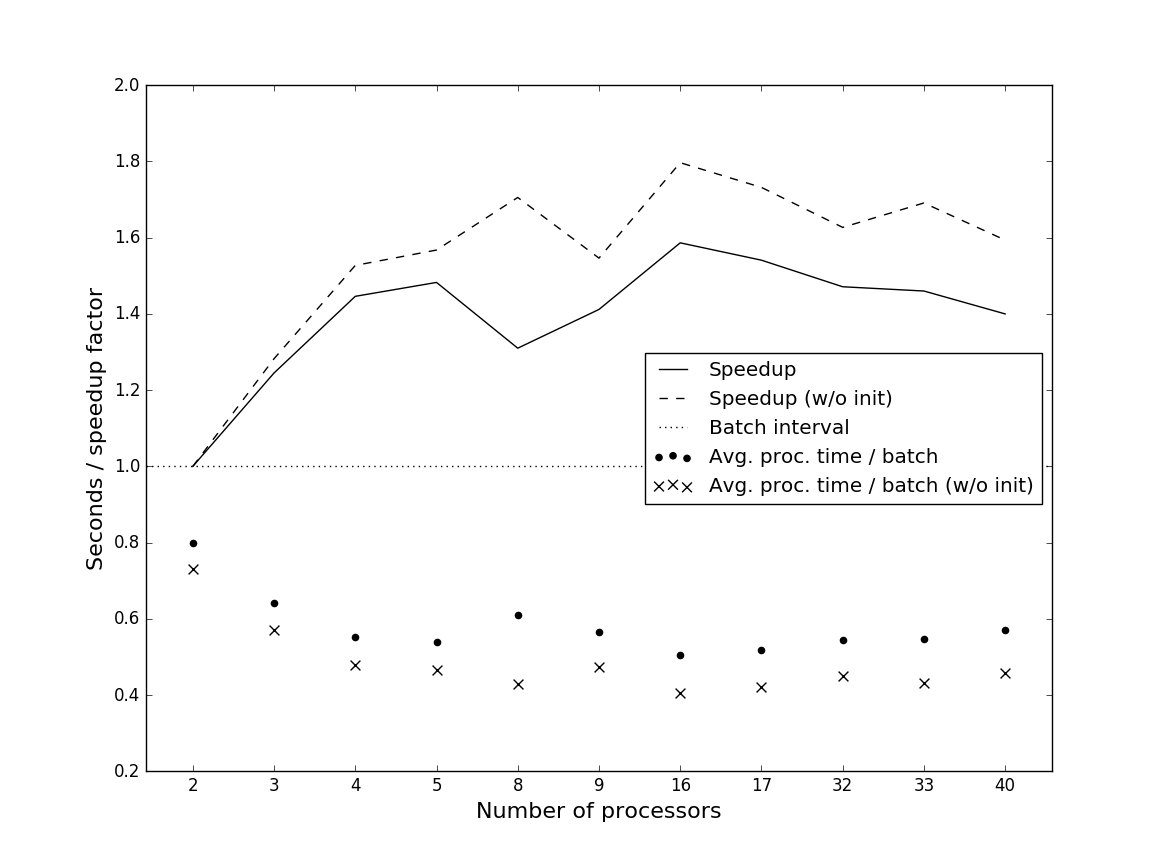
\includegraphics[scale=0.39]{./styles/perf20-2.png}
 \caption{Scalability: Stream speed = 10000, q = 20, d = 2}
 \label{fig:perf20-2}
\end{figure}


The charts here presented show the speedup obtained by increasing the number of processors from 2 to 40, which in reality means that 1 to 39 processors where used for the computations. It also shows the average processing time for each batch of data. Because the initialization takes the most amount of time, it is also convenient to show these values without considering that process: by doing so it is possible to see what would be the expected results for a longer run, where the initialization is no longer dominant. Finally it shows the interval time for which Spark process a new batch of data, in particular all these tests processed batch every second.



\begin{figure}[h!]
 \centering
 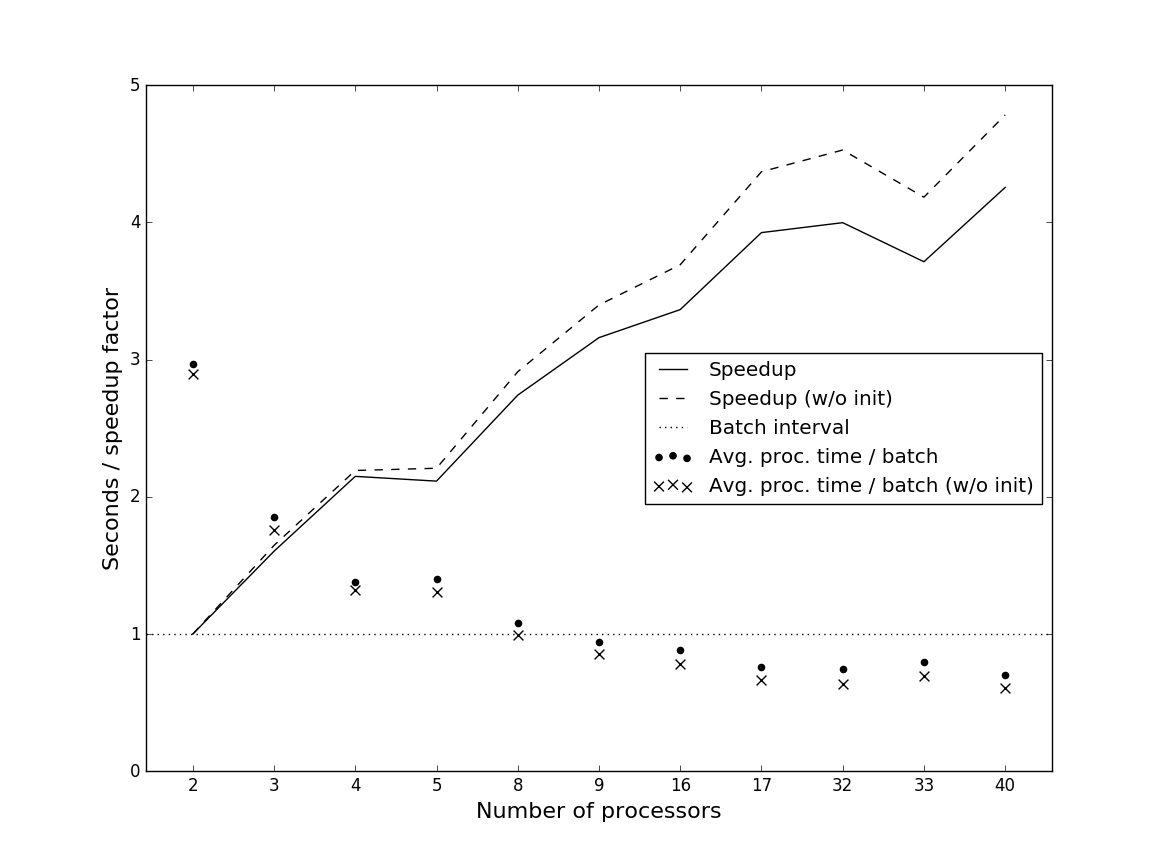
\includegraphics[scale=0.4]{./styles/perf20-100.png}
 \caption{Scalability: Stream speed = 10000, q = 20, d = 100}
 \label{fig:perf20-100}
\end{figure}


Figure \ref{fig:perf20-2} shows that using only 20 micro-clusters and 2 dimensions has poor scalability, not even being able to perform twice as fast as for a single processor (2 in total). Even for this high speed streaming, one processor is enough to process the batches of data before a new batch is processed, meaning that the setup is stable.

\begin{figure}[h!]
 \centering
 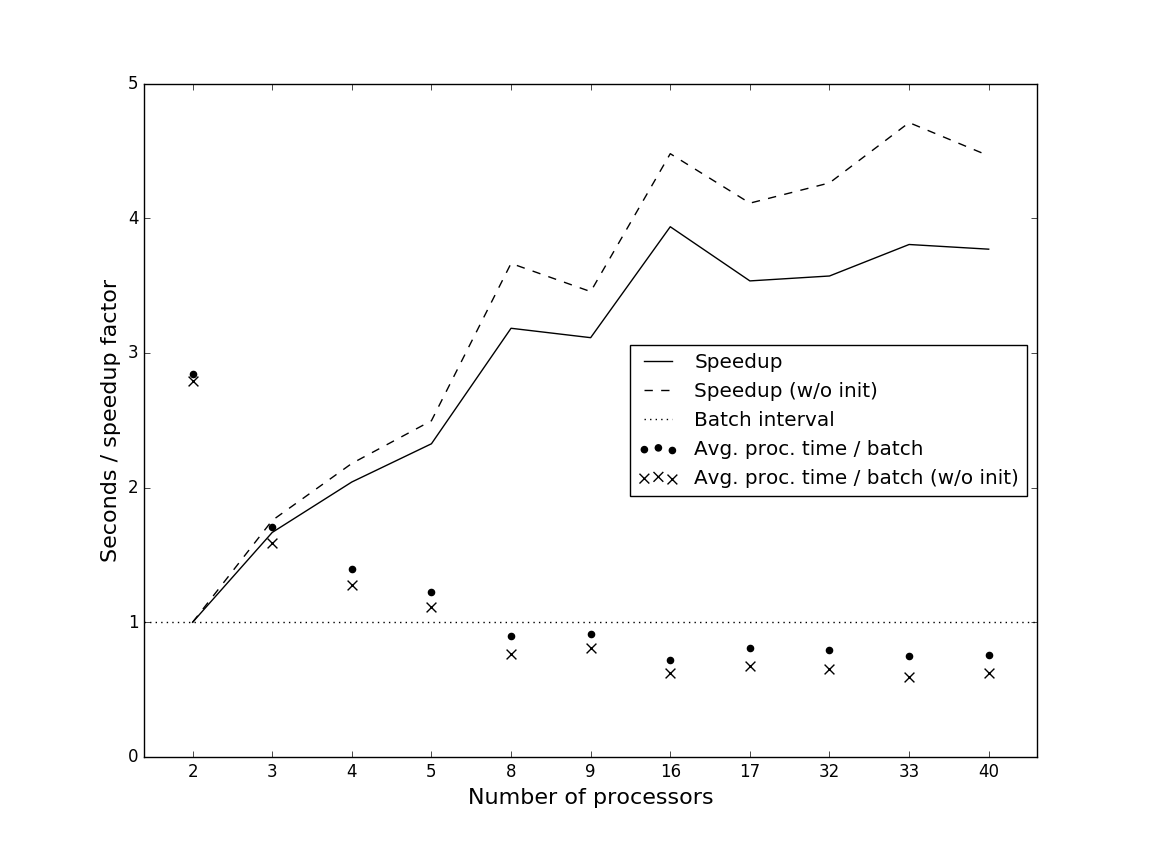
\includegraphics[scale=0.42]{./styles/perf200-2.png}
 \caption{Scalability: Stream speed = 10000, q = 200, d = 2}
 \label{fig:perf200-2}
\end{figure}

Increasing the dimensionality of the points increases the computational effort needed to process the points in every batch of data and here is where \textit{Spark-CluStream} shows its scalability, which is almost linear\footnote{By linear scalability does not mean it scales with a 1 to 1 ratio, but rather linearly proportional.} for up to 16-17 processors, as it can be seen in Figure \ref{fig:perf20-100}.  From the average processing time per batch, it can be seen that from 32 to 40 processors it does not improve much anymore and the speedup does not increase quasi-linearly anymore. Here a total of 9 processors were required to stabilize \textit{Spark-CluStream}. 

\begin{figure}[h!]
 \centering
 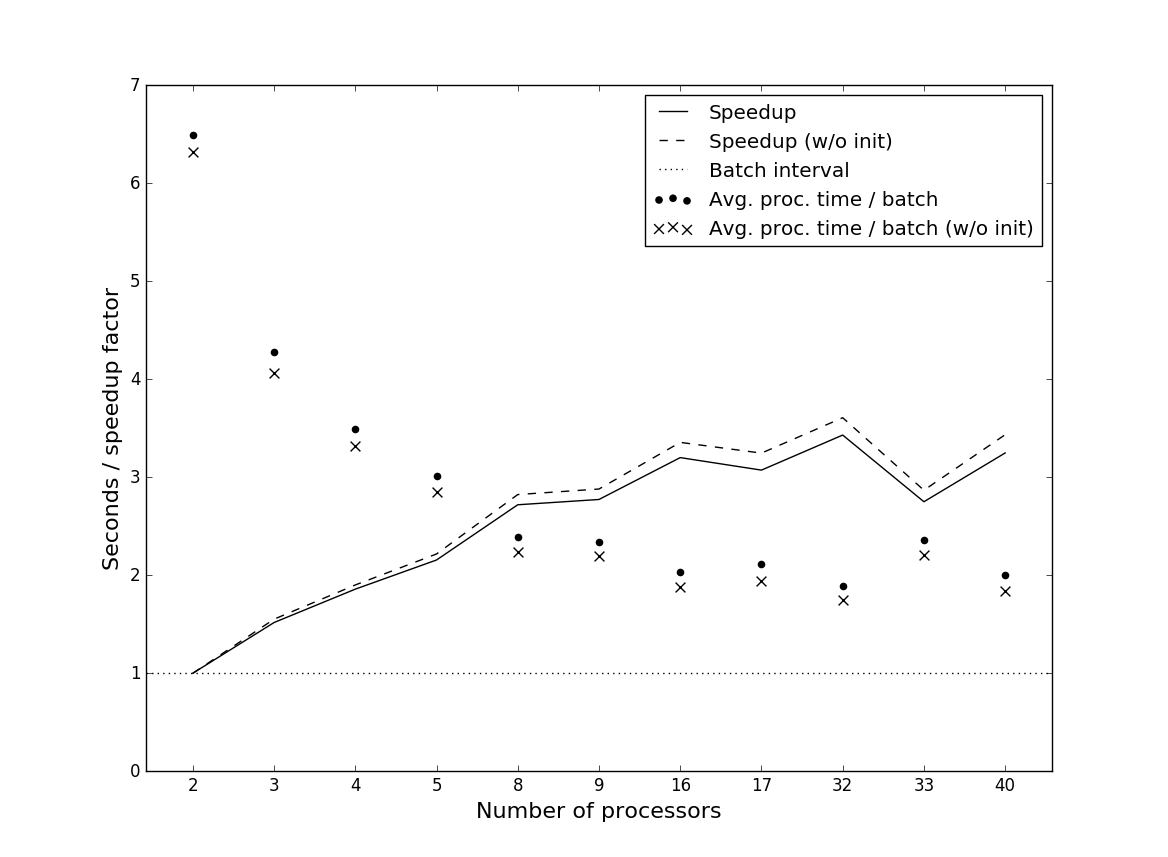
\includegraphics[scale=0.4]{./styles/perf200-100.png}
 \caption{Scalability: Stream speed = 10000, q = 200, d = 100}
 \label{fig:perf200-100}
\end{figure}

Interestingly, increasing the number of micro-clusters by a factor of 10 for 2 attributes resulted in good scalability, similarly to the scenario with 20 micro-clusters and 100 attributes. Here a total of 8 processors were enough for a stable run, as shown in Figure \ref{fig:perf200-2}.



Finally, when the number of clusters and the number of attributes are both increased significantly, Figure \ref{fig:perf200-100} shows for \textit{Spark-CluStream} quasi-linear scalability but this time only up to about 8-9 processors. After that point, the speedup slows down showing almost no improvement after 16 processors. This test never reached a stable configuration.

\subsubsection{Comparison against alternatives}

It is important for this project to know how \textit{Spark-CluStream} stands against some of the other alternatives for stream clustering available for Spark, in particular: \textit{Streaming K-Means} from Spark and \textit{StreamDM-CluStream}, which is another adaptation of the \textit{CluStream} method for Spark. There are two aspects of interest in this tests, one being their clustering capabilities and the other their performance.

\subsection{Clustering}

The setup and the dataset are the same as in \ref{validation}, as having already verified results provides the possibility of using those tests to directly compare the results against the other methods. Again, the used measurement is the sum of squares (SSQ).

Before looking at the results, here are some key considerations for the other methods:

\begin{itemize}
 \item \textit{Streaming K-Means}:
 \begin{itemize}
  \item In order to have comparable results, the time horizon $H$ must be interpreted differently. There are two strategies: the first option is to use the parameter \textit{halfLife}, which can be configured to let the algorithm to completely adjust the clusters after $HL$ points or batches.
  \item The alternative would be to set the $decayFactor$, which sets the weight for the clusters of the "old" data (only the current batch is considered "new" data). This is a number between 0 and 1, such that if it is 0 then only the clusters for "new" data determine the final clusters, if it is set to 1, then the clusters of past data will have the same influence on the final clusters. It is important to notice that this \textit{decayFactor} also considers the number of points of the "new" and "old" data, so in the last case, after a long time, "new" data will have little influence as the number of points of the current batch will be considerable smaller than the points clustered so far.
 \end{itemize}
 \item \textit{StreamDM-CluStream}:
 \begin{itemize}
  \item This adaptation of \textit{CluStream} does not include the offline part as a separate module, meaning that it does not save snapshots and therefore it has to perform the macro-clustering process for every batch. This brings some limitations, the horizon $H$ no longer has the same meaning: the $\delta$ parameter is used instead as an equivalent, relying on the micro-clustering part only and its ability to delete and create new micro-clusters.
\end{itemize}

\end{itemize}

\subsubsection{Case 1}

The parameters used for \textit{Spark-CluStream} are the same as in \ref{validation}. The number of clusters $k$ is always 5 for this dataset and these tests for all methods.

For \textit{Streaming K-Means}, the horizon $H=1$ was transformed to $halfLife=1000$ points. This is because the speed of the stream is 2000 points per time unit, if the horizon is 1, then only 2000 points are desired to be clustered, and half of that results in 1000 points. For the \textit{decayFactor}, it is safe to choose 0, as that would mean that only the last 2000 points have influence on the clusters, which is exactly what it's desired.

\textit{StreamDM-CluStream} is set up with its default parameters, only changing the horizon to 1 and the number of micro-clusters to 50 in order to match those of \textit{Spark-CluStream}.

\begin{figure}[h]
 \centering
 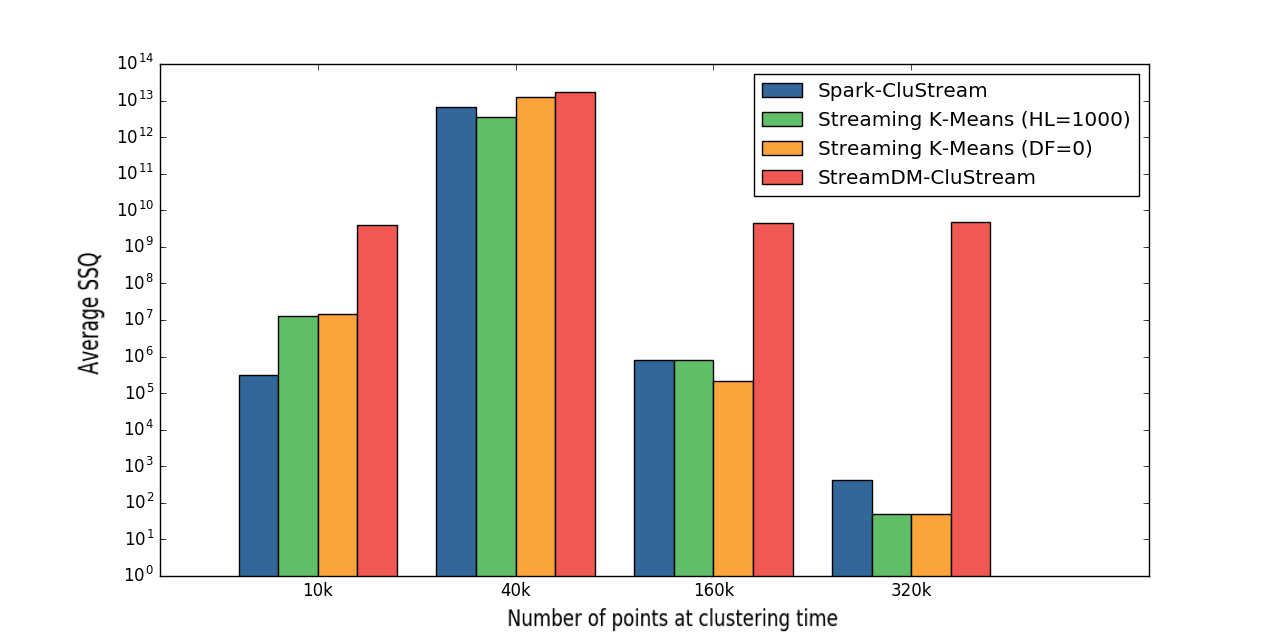
\includegraphics[scale=0.4]{./styles/comparison2000.png}
 \caption{Comparison results: all methods. Stream speed = 2000, H=1}
 \label{fig:comparison2000}
\end{figure}

From Figure \ref{fig:comparison2000} it can be seen that \textit{Spark-CluStream} delivers results which are very close to those of \textit{Streaming K-Means}, which performs significantly better than the older method \textit{STREAM}. Also, \textit{Streaming K-Means} with the \textit{decayFactor} (DF) is expected to do well on this test as it could be configured to cluster exactly as it was intended for this dataset. 

The surprising results came from \textit{StreamDM-CluStream}, as it performed noticeably, and significantly, worse than the rest of the methods. Specially for the last two marks at $160k$ and $320k$ it shows poor performance, which are where the other methods performed the better on average.

To find out whether this behavior is due to not using the snapshots plus offline macro-clustering, another test was performed using \textit{Spark-CluStream} with the same conditions as for \textit{StreamDM-CluStream}: using $\delta = 1$ as the horizon and $m=100$ to match both methods

\begin{figure}[h]
 \centering
 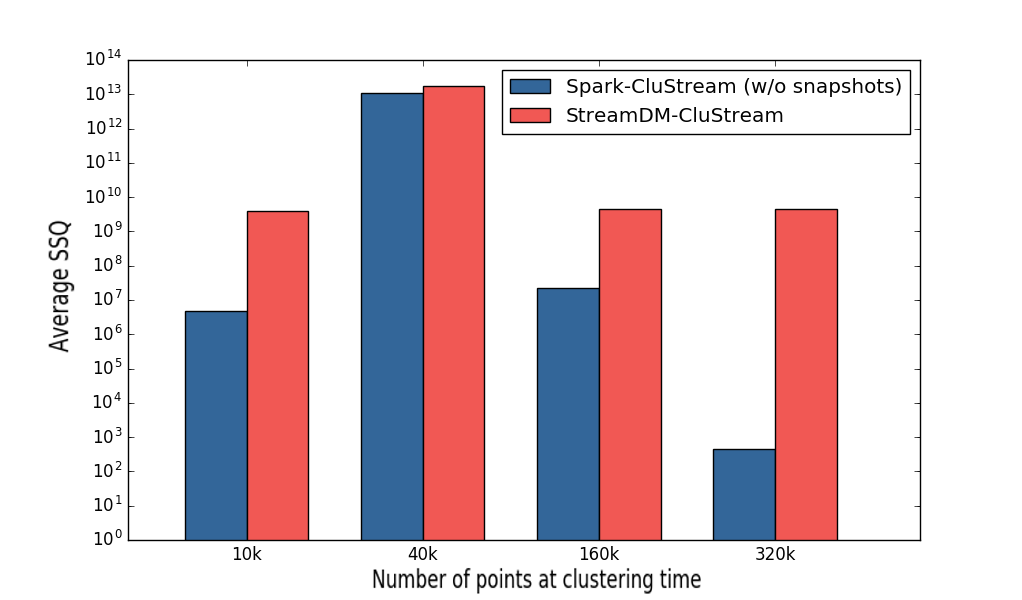
\includegraphics[scale=0.4]{./styles/comparisonNoSnaps.png}
 \caption{\textit{Spark-CluStream} without snapshots. Stream speed=2000, H=1, m=100}
 \label{fig:comparisonNoSnaps}
\end{figure}

Figure \ref{fig:comparisonNoSnaps} shows poorer results for \textit{Spark-CluStream} in comparison to its original behavior with snapshots, but still delivers noticeably better results than \textit{StreamDM-CluStream}, even though all these tests were executed 4 times and the SSQ erros were averaged to get a better representation of how these methods perform.

\subsubsection{Case 2}

Repeating the experiment for the stream with a speed of 200 and a horizon $H=256$ revealed unexpected results. While most parameters for all methods remained the same, for \textit{Streaming K-Means} a new $halfLife$ has to be calculated: multiplying the speed of the stream to the horizon, $200\cdot 256=51200$ shows how many points of the stream are supposed to be clustered at each time, indicating that the parameter should be set to $halfLife=25600$. 

\begin{figure}[h!]
 \centering
 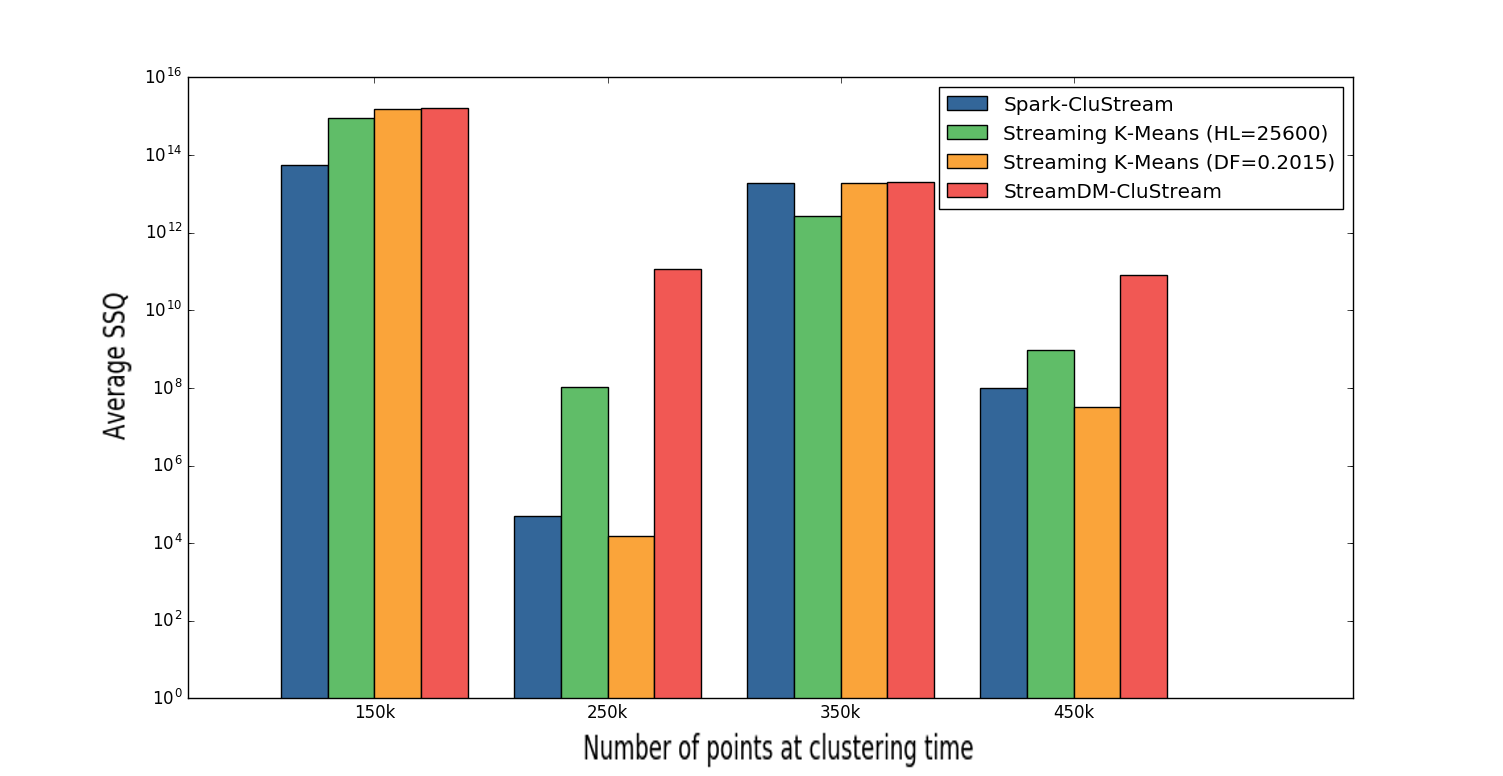
\includegraphics[scale=0.37]{./styles/comparison200.png}
 \caption{Comparison results: all methods. Stream speed = 200, H=256}
 \label{fig:comparison200}
\end{figure}

The \textit{decayFactor} strategy at first seems that does not work for such experiment, but considering that the total number of entries is known and exactly the marks at which the clustering process happens, it is possible to calculate an average value to use as a $decayFactor$: 

\begin{itemize}
 \item At 150000 points: $\frac{51200}{150000} \approx 0.3413$, which is the ratio of the points to cluster to the total number of points at that particular time.
 \item At 150000 points: $\frac{51200}{250000} \approx 0.2048$.
 \item At 150000 points: $\frac{51200}{350000} \approx 0.1462$.
 \item At 150000 points: $\frac{51200}{450000} \approx 0.1137$.
\end{itemize}

Averaging those ratios leads to a \textit{decayFactor = 0.2015}, which is a way to determine how important the old data is in comparison to the new one.


Figure \ref{fig:comparison200} shows that while \textit{Spark-CluStream} still performs consistently good, \textit{Streaming K-Means} with the \textit{decayFactor} outperformed its relative with the $halfLife$ strategy. Another thing to notice is that \textit{StreamDM-CluStream} still delivered the worse results. 

\begin{figure}[h]
 \centering
 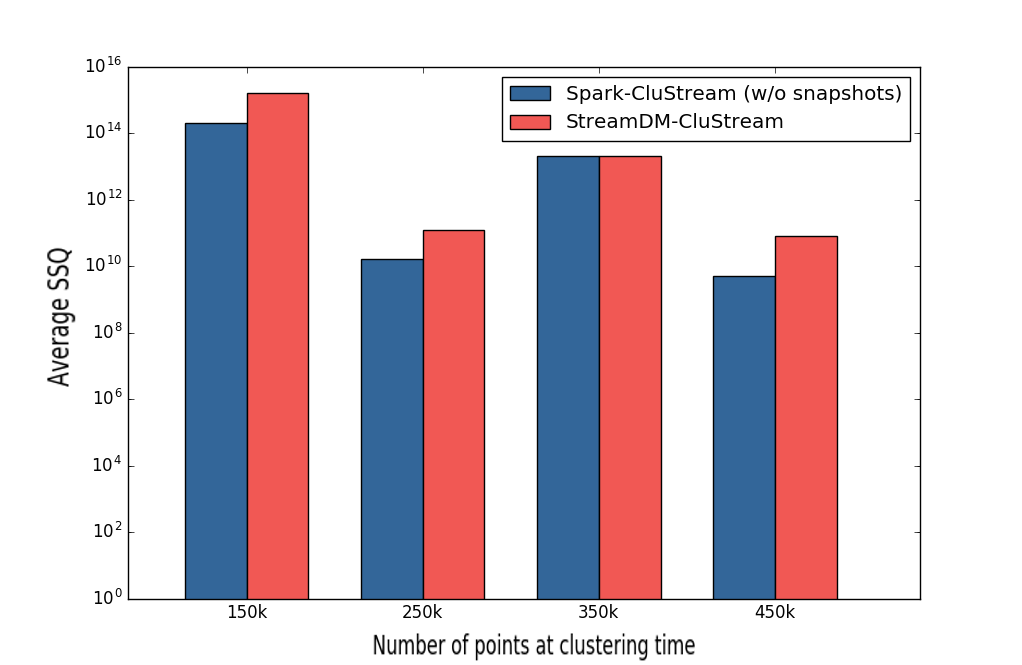
\includegraphics[scale=0.4]{./styles/comparisonNoSnaps2.png}
 \caption{\textit{Spark-CluStream} without snapshots. Stream speed = 200, H=256, m=100}
 \label{fig:comparisonNoSnaps2}
\end{figure}

Testing \textit{Spark-CluStream} again without the use of snapshots, showed once more that it delivers better results than \textit{StreamDM-CluStream}, as it can be seen in Figure \ref{fig:comparisonNoSnaps2}, but the difference was reduced significantly. These results might indicate that \textit{StreamDM-CluStream} does not benefit from shorter horizons.

\subsection{Performance}

In this section, the scalability of \textit{Spark-CluStream} is compared to that of \textit{StreamDM-CluStream} and Spark's \textit{Streaming K-Means} unsing the Spark cluster setup for $q=20$ and $d=2,100$, for the $CluStream$ method. Also, a test on a signle machine is performed, using the setup and dataset as in \ref{validation}.


\begin{figure}[h!]
 \centering
 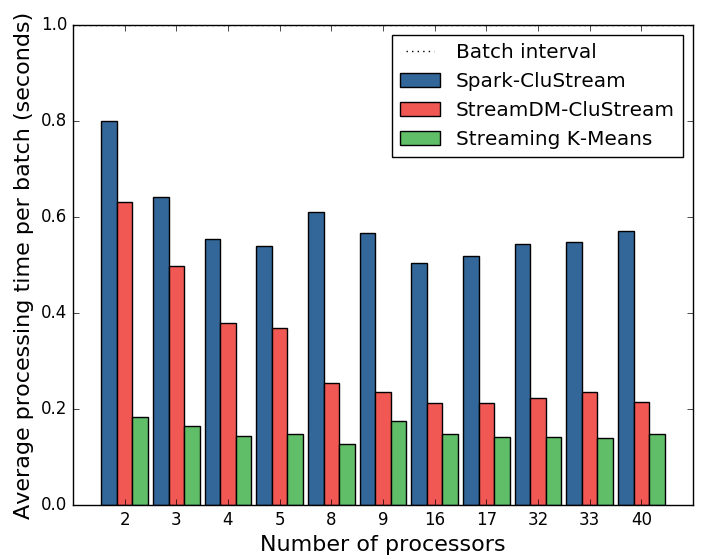
\includegraphics[scale=0.47]{./styles/perfComp2.png}
 \caption{Processing time comparison: $q=20$, $d=2$}
 \label{fig:perfComp2}
\end{figure}

In Figure \ref{fig:perfComp2} it can be seen that \textit{Spark-CluStream} took the most time on average to process a batch of data and being \textit{Streaming K-Means} the fastets among the three. 

\begin{figure}[h!]
 \centering
 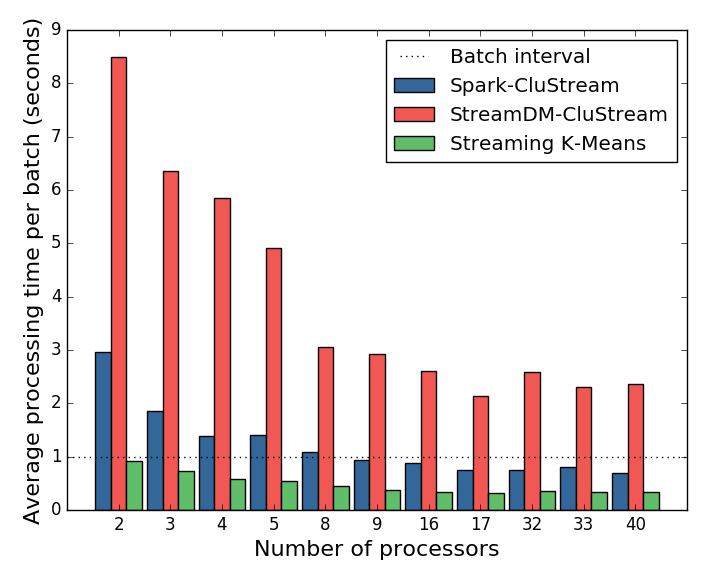
\includegraphics[scale=0.47]{./styles/perfComp100.png}
 \caption{Processing time comparison: $q=20$, $d=100$}
 \label{fig:perfComp100}
\end{figure}

When it comes to higher dimensions, \textit{Spark-CluStream} shows a significant improvement over \textit{StreamDM-CluStream}, which never got to the point were it was stable (below the 1 second mark), as shown in \ref{fig:perfComp100}, it seems to scale as fast as \textit{Spark-CluStream} but it was not enough even with 40 processors. 


\begin{figure}[h!]
 \centering
 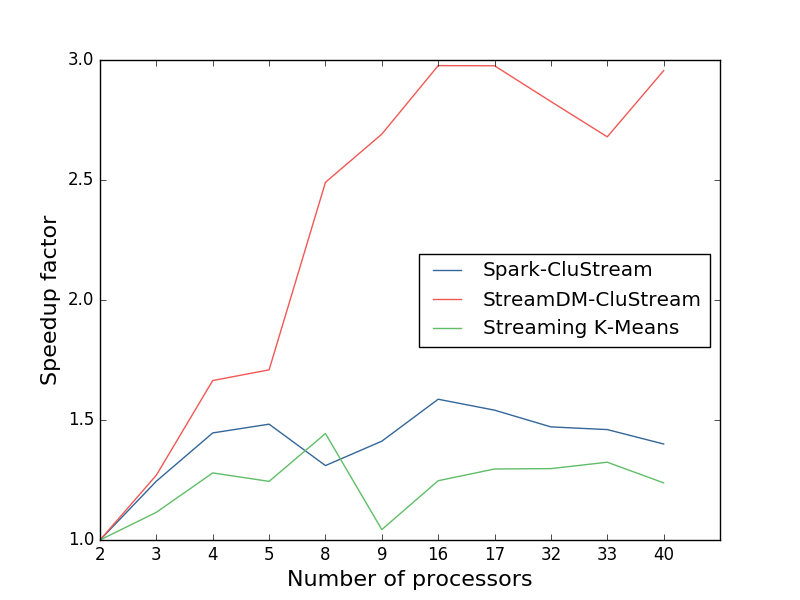
\includegraphics[scale=0.47]{./styles/scalComp2.png}
 \caption{Scalability comparison: $q=20$, $d=2$}
 \label{fig:scalComp2}
\end{figure}

Surprisingly, in Figure \ref{fig:scalComp2}, \textit{StreamDM-CluStream} shows to be able to scale even for this tests, while both \textit{Spark-CluStream} and \textit{Streaming K-Means} seem to struggle taking advantage of using more processors.

\begin{figure}[h!]
 \centering
 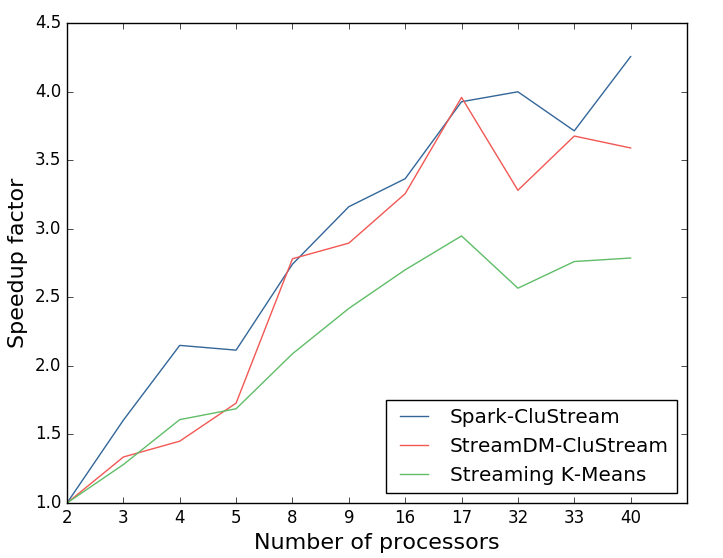
\includegraphics[scale=0.47]{./styles/scalComp100.png}
 \caption{Processing time comparison: $q=20$, $d=100$}
 \label{fig:scalComp100}
\end{figure}

Figure \ref{fig:scalComp100} shows that all three algorithms are able to scale similarly for this test, being \textit{Spark-CluStream} the one having a very slight advantage as it does not slow down as quickly as the other two.



Another interesting comparison, is the processing time per batch of data for a single machine, using a real dataset such as the \textit{Network Intrusion}. Here, communication is less of an issue as all the partitions lie in the same share memory space, and still there are 4 virtual cores in disposition for the algorithms to run. 

The test was performed using a stream speed of 2000 points per batch and with a horizon $H=1$, to match one of the validation tests.

\begin{figure}[h!]
 \centering
 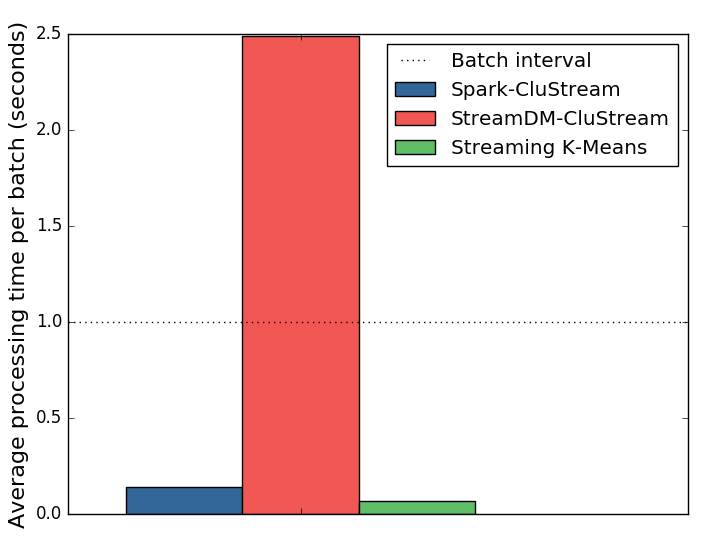
\includegraphics[scale=0.47]{./styles/singlemachine.png}
 \caption{Processing time comparison for a single machine: $q=50$, $d=34$}
 \label{fig:singlemachine}
\end{figure}

The results shown in Figure \ref{fig:singlemachine} are quite remarkable. As \textit{StreamDM-CluStream} shows a very significant disadvantage when using greater numbers of micro-clusters and higher dimensions.

For this single machine test, \textit{Spark-CluStream} was about 18 times faster on average than \textit{StreamDM-CluStream} and about two times slower than \textit{Streaming K-Means} on average.

Another consideration to be made, is that  \textit{Spark-CluStream} saves a snapshot for every batch of data, having to write to disk, while the other two algorithms never access the disk or this matter.



\section{Conclusions}

 
Bringing successfully the \textit{CluStream} method to Spark has provided valuable information about how similar methods could be adapted by reviewing some of the challenges which might occur. It has also provided deep understanding of this method itself and how stream clustering differs from other clustering methods, which might not need to adapt to changing data, of Apache Spark and how distributed systems work in general, but most importantly it has provided the experience to parallelize algorithms for the specific requirements of a given problem and this knowledge itself is applicable to an uncountable number of problems.

The typical workflow for doing so should follow a similar structure: from understanding the problem as described in chapter \ref{theory}, to going through the process of achieving the desired goals as shown in chapters \ref{implementation} and \ref{results}.

\section{Goals review}

It is rewarding to conclude that the goals were met satisfactorily. Here, the conclusions for every one of them.

\subsection{Adapt \textit{CluStream} in Spark (Spark-CluStream)}

This is the main goal of this thesis, and none of the other goals would have been met if this one failed. Adapting \textit{CluStream} in Spark brought many challenges: one being the fact that the streaming library in Spark handles streams as batches and not individual points with time stamps, forcing this adaptation to change a few things that differentiate it from the original method, and the other one being the parallelization of the algorithm in order to take advantage of distributed computing.

Even though this adaptation changed the way data is processed, i.e. processing the stream in batches of data in parallel as much as possible, the results indicate that this was done correctly and the proof of that lies in the validation section \ref{validation}: it showed that it is not only capable of correctly clustering streams of data but it was able to match the quality of the original method described in \cite{clustreamOrig}. It was shown for two different scenarios that this is true, when comparing the errors obtained after replicating the tests done by the authors of \textit{CluStream}.

\subsection{Understanding its advantages and disadvantages}

The second most important goal was to make this adaptation as scalable as possible, and for this reason many tests were made using different scenarios. There are clearly cases where it is not fully scalable, as shown in section \ref{performance}, but for the most part it was shown comparable scalability as some of the alternatives for Spark, including a method native of Spark and a similar method developed by a team from \textit{Huawei} for a set of stream mining algorithms called \textit{StreamDM}.

Some of its limitations were also understood , such as bottlenecks that might reduce the scalability and performance in general, such as:

\begin{itemize}
 \item Outliers: handling with outliers in sequential code is expected to be a bottleneck, depending on the stream, a batch of data might contain points which do not belong to any micro-cluster and therefore, they have to be handled differently. Depending on the number of outliers, in particular the ones which require two micro-clusters to be merged, the total processing time for that batch will be affected negatively. In general there are three situations where this would normally occur: at the beginning of the stream if the initialization is not accurate, when the incoming data is very noisy and when the data dramatically changes.
 \item Communication costs: running in parallel requires certain communication between processing units. This affects the scalability negatively when few computations are required and too many processing units are used, as most of the time will be spent on communication. Also, as shown in the chapter section \ref{performance}, even when it is expected to be scalable, increasing the number of micro-clusters used and the dimensionality of the data results in a bigger amount of information to communicate, and therefore not allowing greater speedups after a certain amount of processing units. 
\end{itemize}

The results also showed that the \textit{Streaming K-Means} algorithm is the fastest among the three tested (highly optimized for Spark), delivering good results in certain scenarios as it does not count with the flexibility of \textit{CluStream} to better fit to evolving streams. \textit{Spark-CluStream} on the other hand, showed that it not only delivers quality clustering, but also outperformed the similar \textit{CluStream} implementation in \textit{StreamDM}. Quality-wise it delivered more consistent and accurate results, and performance-wise it outperformed it in most cases, including one up to around 18 times faster. 



\begin{table}
\caption{This is the example table taken out of {\it The
\TeX{}book,} p.\,246}
\begin{center}
\begin{tabular}{r@{\quad}rl}
\hline
\multicolumn{1}{l}{\rule{0pt}{12pt}
                   Year}&\multicolumn{2}{l}{World population}\\[2pt]
\hline\rule{0pt}{12pt}
8000 B.C.  &     5,000,000& \\
  50 A.D.  &   200,000,000& \\
1650 A.D.  &   500,000,000& \\
1945 A.D.  & 2,300,000,000& \\
1980 A.D.  & 4,400,000,000& \\[2pt]
\hline
\end{tabular}
\end{center}
\end{table}


\paragraph{Notes and Comments.}
The first results on subharmonics were
obtained by Rabinowitz in \cite{rab}, who showed the existence of
infinitely many subharmonics both in the subquadratic and superquadratic
case, with suitable growth conditions on $H'$. Again the duality
approach enabled Clarke and Ekeland in \cite{clar:eke:2} to treat the
same problem in the convex-subquadratic case, with growth conditions on
$H$ only.

Recently, Michalek and Tarantello (see \cite{mich:tar} and \cite{tar})
have obtained lower bound on the number of subharmonics of period $kT$,
based on symmetry considerations and on pinching estimates, as in
Sect.~5.2 of this article.

%
% ---- Bibliography ----
%
\begin{thebibliography}{5}
%
\bibitem {clar:eke}
Clarke, F., Ekeland, I.:
Nonlinear oscillations and
boundary-value problems for Hamiltonian systems.
Arch. Rat. Mech. Anal. 78, 315--333 (1982)

\bibitem {clar:eke:2}
Clarke, F., Ekeland, I.:
Solutions p\'{e}riodiques, du
p\'{e}riode donn\'{e}e, des \'{e}quations hamiltoniennes.
Note CRAS Paris 287, 1013--1015 (1978)

\bibitem {mich:tar}
Michalek, R., Tarantello, G.:
Subharmonic solutions with prescribed minimal
period for nonautonomous Hamiltonian systems.
J. Diff. Eq. 72, 28--55 (1988)

\bibitem {tar}
Tarantello, G.:
Subharmonic solutions for Hamiltonian
systems via a $\bbbz_{p}$ pseudoindex theory.
Annali di Matematica Pura (to appear)

\bibitem {rab}
Rabinowitz, P.:
On subharmonic solutions of a Hamiltonian system.
Comm. Pure Appl. Math. 33, 609--633 (1980)

\end{thebibliography}

%
% second contribution with nearly identical text,
% slightly changed contribution head (all entries
% appear as defaults), and modified bibliography
%

\clearpage
\addtocmark[2]{Author Index} % additional numbered TOC entry
\renewcommand{\indexname}{Author Index}
\printindex
\clearpage
\addtocmark[2]{Subject Index} % additional numbered TOC entry
\markboth{Subject Index}{Subject Index}
\renewcommand{\indexname}{Subject Index}
\input{subjidx.ind}
\end{document}
